\section{Aufgabe 6}
\begin{equation}
R_{SNR,II}(t)=R_I + \left( 2.02 \frac{E_{SN}}{\rho_0} \right) ^{1/5}(t-t_1)^{2/5}
\end{equation}
\begin{equation}
R_I=400 a * 365 \frac{d}{a} * 24 \frac{h}{d} * 60 \frac{min}{h} * 60 \frac{s}{min} * 5000 \frac{km}{s} = 63072000000000 km
\end{equation}
\begin{equation}
u_{SNR,II}(t) = \frac{dR_{SNR,II}(t)}{dt}=\frac{2 * 2.02^{1/5} \left( \frac{E_{SN}}{\rho_0} \right) ^{1/5}}{5(t-t_1)^{3/5}}
\end{equation}
\begin{equation}
p_0 = \left( 1.66 \times 10^{-26} g/cm^3, 1.66 \times 10^{-24} g/cm^3, 1.66 \times 10^{-22} \right)
\end{equation}
\begin{figure}[ht]
\begin{center}
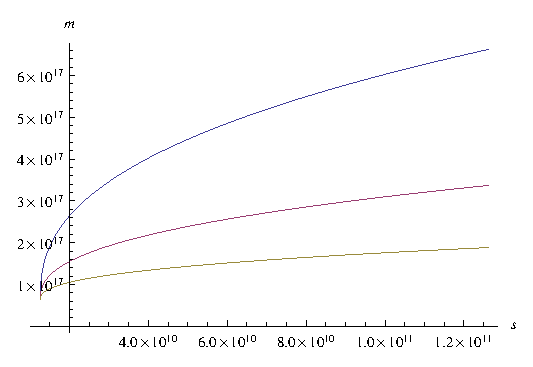
\includegraphics{aufgabe6r.eps}
\end{center}
\end{figure}
\begin{figure}[ht]
\begin{center}
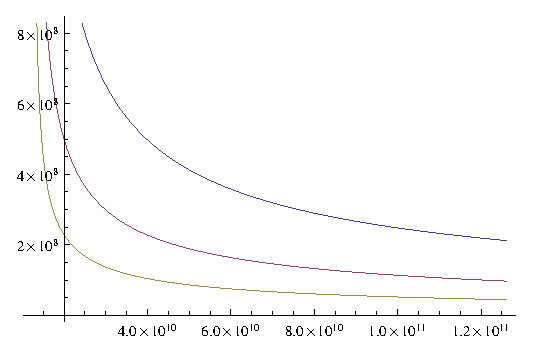
\includegraphics{aufgabe6u.eps}
\end{center}
\end{figure}

